% Template for PLoS
% Version 3.5 March 2018
%
% % % % % % % % % % % % % % % % % % % % % %
%
% -- IMPORTANT NOTE
%
% This template contains comments intended 
% to minimize problems and delays during our production 
% process. Please follow the template instructions
% whenever possible.
%
% % % % % % % % % % % % % % % % % % % % % % % 
%
% Once your paper is accepted for publication, 
% PLEASE REMOVE ALL TRACKED CHANGES in this file 
% and leave only the final text of your manuscript. 
% PLOS recommends the use of latexdiff to track changes during review, as this will help to maintain a clean tex file.
% Visit https://www.ctan.org/pkg/latexdiff?lang=en for info or contact us at latex@plos.org.
%
%
% There are no restrictions on package use within the LaTeX files except that 
% no packages listed in the template may be deleted.
%
% Please do not include colors or graphics in the text.
%
% The manuscript LaTeX source should be contained within a single file (do not use \input, \externaldocument, or similar commands).
%
% % % % % % % % % % % % % % % % % % % % % % %
%
% -- FIGURES AND TABLES
%
% Please include tables/figure captions directly after the paragraph where they are first cited in the text.
%
% DO NOT INCLUDE GRAPHICS IN YOUR MANUSCRIPT
% - Figures should be uploaded separately from your manuscript file. 
% - Figures generated using LaTeX should be extracted and removed from the PDF before submission. 
% - Figures containing multiple panels/subfigures must be combined into one image file before submission.
% For figure citations, please use "Fig" instead of "Figure".
% See http://journals.plos.org/plosone/s/figures for PLOS figure guidelines.
%
% Tables should be cell-based and may not contain:
% - spacing/line breaks within cells to alter layout or alignment
% - do not nest tabular environments (no tabular environments within tabular environments)
% - no graphics or colored text (cell background color/shading OK)
% See http://journals.plos.org/plosone/s/tables for table guidelines.
%
% For tables that exceed the width of the text column, use the adjustwidth environment as illustrated in the example table in text below.
%
% % % % % % % % % % % % % % % % % % % % % % % %
%
% -- EQUATIONS, MATH SYMBOLS, SUBSCRIPTS, AND SUPERSCRIPTS
%
% IMPORTANT
% Below are a few tips to help format your equations and other special characters according to our specifications. For more tips to help reduce the possibility of formatting errors during conversion, please see our LaTeX guidelines at http://journals.plos.org/plosone/s/latex
%
% For inline equations, please be sure to include all portions of an equation in the math environment.  For example, x$^2$ is incorrect; this should be formatted as $x^2$ (or $\mathrm{x}^2$ if the romanized font is desired).
%
% Do not include text that is not math in the math environment. For example, CO2 should be written as CO\textsubscript{2} instead of CO$_2$.
%
% Please add line breaks to long display equations when possible in order to fit size of the column. 
%
% For inline equations, please do not include punctuation (commas, etc) within the math environment unless this is part of the equation.
%
% When adding superscript or subscripts outside of brackets/braces, please group using {}.  For example, change "[U(D,E,\gamma)]^2" to "{[U(D,E,\gamma)]}^2". 
%
% Do not use \cal for caligraphic font.  Instead, use \mathcal{}
%
% % % % % % % % % % % % % % % % % % % % % % % % 
%
% Please contact latex@plos.org with any questions.
%
% % % % % % % % % % % % % % % % % % % % % % % %

\documentclass[10pt,letterpaper]{article}
\usepackage[top=0.85in,left=2.75in,footskip=0.75in]{geometry}

% amsmath and amssymb packages, useful for mathematical formulas and symbols
\usepackage{amsmath,amssymb}

% Use adjustwidth environment to exceed column width (see example table in text)
\usepackage{changepage}

% Use Unicode characters when possible
\usepackage[utf8x]{inputenc}

% textcomp package and marvosym package for additional characters
\usepackage{textcomp,marvosym}

% cite package, to clean up citations in the main text. Do not remove.
\usepackage{cite}

% Use nameref to cite supporting information files (see Supporting Information section for more info)
\usepackage{nameref,hyperref}

% line numbers
\usepackage[right]{lineno}

% ligatures disabled
\usepackage{microtype}
\DisableLigatures[f]{encoding = *, family = * }

% color can be used to apply background shading to table cells only
\usepackage[table]{xcolor}

% array package and thick rules for tables
\usepackage{array}

% create "+" rule type for thick vertical lines
\newcolumntype{+}{!{\vrule width 2pt}}

% create \thickcline for thick horizontal lines of variable length
\newlength\savedwidth
\newcommand\thickcline[1]{%
  \noalign{\global\savedwidth\arrayrulewidth\global\arrayrulewidth 2pt}%
  \cline{#1}%
  \noalign{\vskip\arrayrulewidth}%
  \noalign{\global\arrayrulewidth\savedwidth}%
}

% \thickhline command for thick horizontal lines that span the table
\newcommand\thickhline{\noalign{\global\savedwidth\arrayrulewidth\global\arrayrulewidth 2pt}%
\hline
\noalign{\global\arrayrulewidth\savedwidth}}


% Remove comment for double spacing
%\usepackage{setspace} 
%\doublespacing

% Text layout
\raggedright
\setlength{\parindent}{0.5cm}
\textwidth 5.25in 
\textheight 8.75in

% Bold the 'Figure #' in the caption and separate it from the title/caption with a period
% Captions will be left justified
\usepackage[aboveskip=1pt,labelfont=bf,labelsep=period,justification=raggedright,singlelinecheck=off]{caption}
\renewcommand{\figurename}{Fig}

% Use the PLoS provided BiBTeX style
\bibliographystyle{plos2015}

% Remove brackets from numbering in List of References
\makeatletter
\renewcommand{\@biblabel}[1]{\quad#1.}
\makeatother



% Header and Footer with logo
\usepackage{lastpage,fancyhdr,graphicx}
\usepackage{epstopdf}
%\pagestyle{myheadings}
\pagestyle{fancy}
\fancyhf{}
%\setlength{\headheight}{27.023pt}
%\lhead{\includegraphics[width=2.0in]{PLOS-submission.eps}}
\rfoot{\thepage/\pageref{LastPage}}
\renewcommand{\headrulewidth}{0pt}
\renewcommand{\footrule}{\hrule height 2pt \vspace{2mm}}
\fancyheadoffset[L]{2.25in}
\fancyfootoffset[L]{2.25in}
\lfoot{\today}

%% Include all macros below

\newcommand{\lorem}{{\bf LOREM}}
\newcommand{\ipsum}{{\bf IPSUM}}

%% END MACROS SECTION

% -- my additions --

\usepackage{gensymb}
\usepackage{xspace}

\newcommand{\ca}{$\alpha$-carbon\xspace}
\newcommand{\cas}{$\alpha$-carbons\xspace}

\begin{document}
\vspace*{0.2in}

% Title must be 250 characters or less.
\begin{flushleft}
{\Large
\textbf\newline{Protein structure search to assist protein structure prediction} % Please use "sentence case" for title and headings (capitalize only the first word in a title (or heading), the first word in a subtitle (or subheading), and any proper nouns).
}
\newline
% Insert author names, affiliations and corresponding author email (do not include titles, positions, or degrees).
\\
Ronald Ayoub\textsuperscript{1*},
Yugyung Lee\textsuperscript{1}
\\
\bigskip
\textbf{1} School of Computing and Engineering, University of Missouri at Kansas City, Kansas City, USA
\\
\bigskip

% Insert additional author notes using the symbols described below. Insert symbol callouts after author names as necessary.
% 
% Remove or comment out the author notes below if they aren't used.
%
% Primary Equal Contribution Note
%\Yinyang These authors contributed equally to this work.

% Additional Equal Contribution Note
% Also use this double-dagger symbol for special authorship notes, such as senior authorship.
%\ddag These authors also contributed equally to this work.

% Current address notes
%\textcurrency Current Address: Dept/Program/Center, Institution Name, City, State, Country % change symbol to "\textcurrency a" if more than one current address note
% \textcurrency b Insert second current address 
% \textcurrency c Insert third current address

% Deceased author note
%\dag Deceased

% Group/Consortium Author Note
%\textpilcrow Membership list can be found in the Acknowledgments section.

% Use the asterisk to denote corresponding authorship and provide email address in note below.
* ronaldayoub@mail.umkc.edu

\end{flushleft}
% Please keep the abstract below 300 words
\section*{Abstract}
Lorem ipsum dolor sit amet, consectetur adipiscing elit. Curabitur eget porta erat. Morbi consectetur est vel gravida pretium. Suspendisse ut dui eu ante cursus gravida non sed sem. Nullam sapien tellus, commodo id velit id, eleifend volutpat quam. Phasellus mauris velit, dapibus finibus elementum vel, pulvinar non tellus. Nunc pellentesque pretium diam, quis maximus dolor faucibus id. Nunc convallis sodales ante, ut ullamcorper est egestas vitae. Nam sit amet enim ultrices, ultrices elit pulvinar, volutpat risus.


% Please keep the Author Summary between 150 and 200 words
% Use first person. PLOS ONE authors please skip this step. 
% Author Summary not valid for PLOS ONE submissions.   
\section*{Author summary}
Lorem ipsum dolor sit amet, consectetur adipiscing elit. Curabitur eget porta erat. Morbi consectetur est vel gravida pretium. Suspendisse ut dui eu ante cursus gravida non sed sem. Nullam sapien tellus, commodo id velit id, eleifend volutpat quam. Phasellus mauris velit, dapibus finibus elementum vel, pulvinar non tellus. Nunc pellentesque pretium diam, quis maximus dolor faucibus id. Nunc convallis sodales ante, ut ullamcorper est egestas vitae. Nam sit amet enim ultrices, ultrices elit pulvinar, volutpat risus.

\linenumbers

% Use "Eq" instead of "Equation" for equation citations.
\section*{Introduction}

Determining the structure of a protein is an important step towards understanding its function.
Current experimental structure determination methods such as X-ray crystallography and nuclear magnetic resonance (NMR) are resource intensive and timing consuming.
Given the higher throughput of current sequencing methods, experimental protein structure determination is unable to keep pace.
Being able to predict a protein structure from its amino acid sequence would address this problem. 
However, protein structure prediction remains a central unsolved problem in molecular biology. 

CASP is a biannual blind competition for protein structure prediction that began in 1994 \cite{Moult1995}.
Progress has been slow until the success of coevolutionary methods in contact prediction demonstrated in CASP11 \cite{Moult2016}.
Now, the recent success of AlphaFold at CASP13 \cite{alq2019} using deep learning combined with coevolutionary methods has refocused interest on the problem. 
While AlphaFold's performance was remarkable, the problem remains largely unsolved and more work remains to be done \cite{alq2019}. 

In \cite{Ayoub2019} we introduced RUPEE, a purely geometric protein structure search with no dependence on sequences, clustering, and pre-calculated results. 
We compared our results with the mTM-align structure search \cite{Dong2018}, the secondary structure matching (SSM) search \cite{Krissinel2004}, and the CATHEDRAL structural scan \cite{Redfern2007}, and found RUPEE is equal to or better than the best available structure searches on a benchmark of known protein domains. 
Additionally, we showed RUPEE, on average, is able to return results faster than mTM-align and CATHEDRAL. 

Since the release of RUPEE, we have observed that the primary usage pattern for RUPEE has been to upload protein structures that have a very low maximum similarity to other structures in the PDB.
In most cases, these uploaded protein structures are the output of a protein structure prediction protocol. 
While in \cite{Ayoub2019} we recognized the desirability of a purely geometric protein structure search, we did not anticipate the utility of such a search to aid in the development of protein structure prediction methods.
For instance, besides measuring the similarity of a predicted structure to a target structure in order to evaluate a protein structure prediction method in development, it is also natural to determine what known structure a predicted structure resembles most. 

[got here in my second pass]
Recognizing the need for being able to search on query structures with low maximum similarity to known structures, we have added an additional search mode to RUPEE with increased sensitivity. 
While top-aligned mode, introduced in \cite{Ayoub2019}, is comparitively good for low similarity searches, the all-aligned mode we introduce below provides a significant improvement over top-aligned mode in that case.  
In this paper, we again compare RUPEE's results mTM-align, SSM, and CATHEDRAL but this time we do so for all-aligned mode and we derive a benchmark from free-modelling predictions in CASP12. 
Whereas in \cite{Ayoub2019} we showed that RUPEE is equal or better than those we compared to for a benchmark of known protein structures, in this paper we show that RUPEE, in all-aligned mode, is clearly better than those we compare to using a benchmark drawn from the structures output by protein structure prediction protocols. 

Originally, the RUPEE protein structure search focused on full-length matches. 
If you wanted to search for structures similar to a domain, you could search one of the protein domain classification databases such as SCOPe, CATH, or ECOD.
On the other hand, if you wanted to search for structures similar to a whole chain, you could search whole chains from the PDB. 
While the ability of RUPEE to search multiple databases for any given structure is flexible, adding the ability to execute containment searches extends this flexibility.
Therefore, RUPEE now supports explicit search types for \emph{Contained-In} and \emph{Contains} searches in addition to the \emph{Full-Length} search type.

Together, all-aligned mode and containment searches are siginificant additions to RUPEE that increase its utility and further demonstrates the advantage of a purely geomietric protein structure search without dependencies on sequence, precalculated results or clustering.

\section*{Related work}

Pairwise alignment involves finding a set of spatial rotations and translations for two protein structures that minimizes a distance metric. 
Traditionally, the root mean squared deviation (RMSD) between \cas of aligned residues is minimized.
However, the RMSD score does not factor in the distance between unaligned residues nor does it consider the percentage of aligned residues, that is, alignment \emph{coverage}. 
RMSD scores also have some dependence on the length of the aligned proteins. 
On the other hand, the TM-score \cite{Zhang2004} takes all residues into account and normalizes for both coverage and length of the aligned proteins. 
For this reason, TM-score is frequently used in the assessment of protein structure alignments. 

Pairwise alignments often favor accuracy over speed because the typical use case of aligning one protein structure to another does not impose tight response time requirements. 
On the other hand, a protein structure search can involve thousands of comparisons and accuracy is often balanced against speed. 
In this case, pairwise alignment is still useful for evaluating the results of a search, and this is the approach we take. 

For pairwise alignment, Combinatorial Extensions (CE) \cite{Shindyalov1998} and FATCAT \cite{Ye2003} are among the most popular tools, representing rigid and flexible protein alignments, respectively. 
CE performs a rigid alignment in order to minimize RMSD and FATCAT allows for a constrained number of twists in the protein chain in order to find a more flexible alignment before minimizing RMSD.

Besides CE and FATCAT, TM-align \cite{Zhang2005} and DALI \cite{Sander1995} are pairwise alignment tools also in wide use, both offering their own distinct approaches to structure alignment. 
TM-align uses a rotation matrix designed to maximize the TM-score rather than minimizing the RMSD along with dynamic programming to find the best full-length alignment. 
DALI compares intramolecular distance matrices between two proteins to find a consistent set of matched submatrices that is used to align the proteins. 

Of the pairwise alignment tools, CE, FATCAT, TM-align and DALI, we have found TM-align is the fastest while also providing high-quality pairwise structure alignments. 
It is for this reason that we use TM-align for RUPEE.

Whereas pairwise structure alignments only depend on the sequence of \ca coordinates, protein structure searches often introduce a further dependence on the sequence order of amino acids.
This approach often takes the form of clustering proteins based on sequences and pre-calculating results for pairwise alignments among cluster representatives. 
Then, these pre-calculated results are used for filtering the number of structures used for comparisons against a query protein.
The exact formula for combining the use of representatives and pre-calculated results varies from system to system.
However, all systems using this approach share the same disadvantage, an indirect dependence on amino acid sequences. 
In the absence of a reliance on sequence representatives and pre-calculated results, and without sacrificing accuracy, response times suffer greatly, often taking upwards of an hour for queries to complete. 

For protein structure searches, VAST \cite{Gilbrat1996} and the FATCAT server \cite{Ye2004} are among the most popular. 
Nonetheless, these searches are slow in comparison to the structure searches we compare to in this paper, mTM, SSM, and CATHEDRAL, when pre-calculated results are not used. 
If given a known protein domain, VAST can return structural neighbors in seconds using pre-calculated results. 
However, if uploading a PDB file where pre-calculated results are not used, response times for VAST can exceed 30 minutes. 
Similarly, the FATCAT server, that does not use pre-calculated results, can take over an hour to send results for a search against PDB-90 representatives \cite{Prlic2010}. 

DALI also provides a heuristic structure search \cite{Holm2010} of whole chains found in the PDB in addition to a tool for pairwise structure alignments using distance matrices as discussed above. 
In the case of searching, DALI first identifies matched PDB-90 representatives and then walks a pre-calculated graph of structural similarities to identify further matches in the PDB to gradually build up the set of structures similar to the query structure. 
DALI is slow in comparison to SSM, and mTM has shown better quality results than DALI \cite{Dong2018}.

[Note: add how the need for protein structure prediction is needed extra accuracy. ]


Given the above, there remains a need for a purely geometric protein structure search.
For the serendipitous exploration of relations between protein structures performed in the trenches, this search should be fast. 
Moreover, with a $~10\%$ yearly growth rate of solved structures deposited in the PDB \cite{gkw1000}, this search should be scalable. 
At a minimum, RUPEE takes a significant step in this direction as will be shown below. 

These requirements were satisifed in \cite{Ayoub2019}. However, this is also a need for higher sensitivity / greater accuracy when it comes to protein structure prediciton output and protein design.  

\section*{Methods}

[NOTE: this assumes we have introduced top-aligned mode and all-aligned mode in the introduction]

We first provide a brief outline of our linear encoding of protein structures described in more detail in \cite{Ayoub2019}, which still remains at the core of the RUPEE protein structure search. 
Then, we describe the types of similarity scores used for the initial filtering in the different search modes, the addition of search types, changes to top-aligned mode, and the addition of all-aligned mode, in that order.

\subsection*{Linear encoding of protein structure}

In \cite{Ayoub2019}, we introduced a linear encoding of protein structures.
For each pair of torsion angles combined with their secondary structure assignment, we assign an integer we refer to as a residue descriptor.
For instance, a $\beta$-turn-$\beta$ motif may be represented as a sequence of residue descriptors, similar to that shown below. 
\begin{gather}\label{E:descrseq} 
    [\, 5, 5, 5, 5, 5, 5, 7, 5, 11, 11, 5, 5, 5, 5, 5, 5 \,]
\end{gather}

Next, we derive a multiset of overlapping 3-grams of residue descriptors. 
This representation is often referred to as shingling and was developed in \cite{Broder1997a}. 
The overlap between shingles ensures some of the order information within the original sequence is preserved in the multiset. 

By shingling, we obtain a multiset of ordered lists from an ordered list of residue descriptors. 
As an example, the sequence in (\ref{E:descrseq}) becomes the following multiset of shingles. 
\begin{align}\label{E:shinglebag}
    \begin{split}
        \{\,&[5, 5, 5], [5, 5, 5], [5, 5, 5], [5, 5, 5], [5, 5, 7] \\
            & [5, 7, 5], [7, 5, 11], [5, 11, 11], [11, 11, 5], [11, 5, 5] \\
            & [5, 5, 5], [5, 5, 5], [5, 5, 5], [5, 5, 5] \,\}
    \end{split}
\end{align}

Next, each shingle $s$ is hashed to an integer as shown in~(\ref{E:hashdef}). 
\begin{gather}\label{E:hashdef}
    s_{hash} = s_1 \times 13^2 + s_2 \times 13 + s_3
\end{gather}

After hashing, the multiset in (\ref{E:shinglebag}) becomes the following multiset of integers.
\begin{align}\label{E:hashbag}
    \begin{split}
    \{\,&915, 915, 915, 915, 917, 941, 1259 \\
        &999, 2007, 1929, 915, 915, 915, 915 \,\}
    \end{split}
\end{align}

The hashing completes the transformation of an ordered list of residue descriptors to a multiset of integers that still retains some of the order information present in the original list. 

Notice in (\ref{E:hashbag}) the value 915, corresponding to the shingle $[ 5, 5, 5 ]$, occurs frequently indicating the presence of $\beta$-strands. 
To address this lack of specificity, we introduced a heuristic we call \emph{run position encoding} (RPE), where a run is a consecutive sequence of identical descriptors. 
To distinguish between short and long runs, thereby increasing the specificity of the shingles, we add a factor of $10^5$ to each shingle hash as a function of the first residue's position in a run. 
Applying to the multiset of integers in (\ref{E:hashbag}) gives
\begin{align}\label{E:rpebag}
    \begin{split}
    \{\,&00915, 10915, 20915, 20915, 10917, 00941, 01259 \\
        &00999, 02007, 01929, 00915, 10915, 20915, 20915 \,\}
    \end{split}
\end{align}
where the leading zero run factors are shown for clarity. 

The pyramidal approach for the run factors preserves matches at the boundaries between secondary structure runs and loops that would not otherwise be preserved in the presence of differences in run lengths of one or more. 

\subsection*{Similarity scores}

In one case, RUPEE uses the multiset-of-integers representation of protein structures as shown in (\ref{E:rpebag}), and in another case RUPEE regards this multiset as an ordered list of integers.  
We describe the context in which these cases occur in subsequent sections below, but first, we discuss the similarity scores that RUPEE uses for each representation. 

When representing each protein structure using a multiset of integers as shown in (\ref{E:rpebag}), full-length similarity for a candidate pair of structures $a$ and $b$ is defined using the Jaccard similarity \cite{Levan1971} for multisets,
\begin{align}
    J(a,b) = \frac{\sum_i min(a_i, b_i)}{\sum_i max(a_i,b_i)}\text{,}
\end{align}
where $i$ ranges over all possible shingle hashes $s_i$ and $a_i$ and $b_i$ give the counts of shingle hash $s_i$ in structures $a$ and $b$, respectively. 
In words, the Jaccard similarity is the proportion of matched shingles to the total number of shingles. 

When regarding the multiset in (\ref{E:rpebag}) as an ordered list of integers, we assign a pair of protein structures a full-length similarity score using a simplified Needleman-Wunsch \cite{Needleman1970} dynamic programming algorithm where mismatches and gaps are penalized -1 points and matches are awarded +1 points.

\subsection*{Search types}

Originally, the RUPEE protein structure search focused on full-length matches. 
If you wanted to search for structures similar to a domain, you could search one of the protein domain classification databases such as SCOPe, CATH, or ECOD.
On the other hand, if you wanted to search for structures similar to a whole chain, you could search whole chains from the PDB. 
While the ability of RUPEE to search multiple databases for any given structure is flexible, adding the ability to execute containment searches extends this flexibility.
Therefore, RUPEE now supports explicit search types for \emph{Contained-In} and \emph{Contains} searches in addition to the \emph{Full-Length} search type.

In the case where we regard the multiset in (\ref{E:rpebag}) as an ordered list of integers, we score containment using the same simplified Needleman-Wunsch \cite{Needleman1970} algorithm we use for full-length similarity with one small change. 
For containment searches, depending on whether or not the search type is Contained-In or Contains, one of the sides of the dynamic programming matrix is not penalized for the opening gap and end gap.
This is often referred to as semi-global alignment and was developed in \cite{Brudno2003}. 
As it turns out, semi-global alignment is a natural fit for containment comparisons as long as the directionality of containment is explicit. 

\subsection*{Top-aligned mode}

For top-aligned mode, RUPEE uses min-hashing \cite{Broder1998} and locality sensitive hashing (LSH) \cite{Indyk1998} as described in detail in our previous work \cite{Ayoub2019} to quickly estimate the Jaccard similarity of a query protein against all available structures in the searched database.  
Then, the top scoring 40000 protein structures are obtained based on the Jaccard similarity estimates to complete the initial filtering. 

After the initial filtering, we obtain more accurate similarity scores for the filtered matches using the simplified Needleman-Wunsch algorithm. 
Here, the dynamic programming matrix for Needleman-Wunsch is scored as described above based on the chosen search type, Contained-In, Contains, or Full-Length. 
Then, we execute TM-align on the top scoring 8000 matches from Needleman-Wunsch using a reduced number of dynamic programming iterations in the TM-align algorithm. 
We sort these initial alignments by TM-score and obtain the top 400 matches.
Finally, we execute TM-align using the default number of dynamic programming iterations on the top 400 matches and return the results sorted by TM-score. 

In addition to using global or semi-global alignment with the Needleman-Wunsch algorithm, for full-length and containment search types respectively, we also apply the same logic to how normalization is used in the TM-align algorithm. 
For the Full-Length searches we normalize by the average length of both structures, for Contained-In searches we normalize by the query structure and for Contains searches we normalize by the matched structure.
The 3 types of normalization available in TM-align and how they affect searches are discussed in greater detail in the results section of \cite{Ayoub2019}.

The filter sizes of 40000, 8000 and 400 have been chosen based on quality of results and speed. 
We have found that increasing the size of either of these filters results in only marginal improvements in the quality of results. 
Given that performing pairwise alignments is the most time-consuming aspect of the RUPEE structure search, the marginal improvements gained from larger filter sizes have to be balanced against the number of pairwise alignments performed. 

\subsection*{All-aligned mode}

While top-aligned search mode may be sufficient for searching for known protein structures, as was shown in \cite{Ayoub2019} and will also be reinforced below, the need for greater sensitivity arises when searching with structures output from protein structure prediction protocols, where the resultant structure may only have a maximum TM-score of less than 0.50 when compared against all available structures.
Furthermore, for top-aligned mode, the initial filtering is based on full-length matches using the Jaccard similarities, which is not suitable for containment searches. We address both of these concerns by the addition of all-aligned mode. 

The first difference between all-aligned and top-aligned modes is that all-aligned modes skips the min-hashing and LSH step. 
This has the effect of reducing the scalability of all-aligned mode. 
However, we have found that with the current sizes of protein structure databases still being less than a million structures, fast alignments estimates can still be performed on the entire collection using effective multithreading and return within a reasonable amount of time, more often less than 10 minutes on structures with 300 or few residues. 

[I'm not sure if distinguished between TM-align and NW algorithms above in terms of NW being much faster than TM-align.
perhaps this can be done in related work].

% Place figure captions after the first paragraph in which they are cited.
\begin{figure*}[!h]
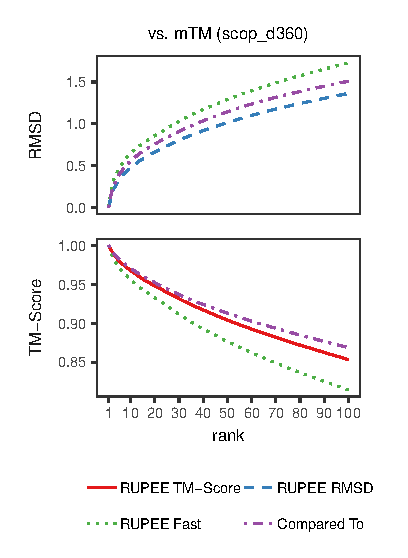
\includegraphics{Fig5}
\caption{{\bf Bold the figure title.}
Figure caption text here, please use this space for the figure panel descriptions instead of using subfigure commands. A: Lorem ipsum dolor sit amet. B: Consectetur adipiscing elit.}
\label{fig5}
\end{figure*}

% For figure citations, please use "Fig" instead of "Figure".
Nulla mi mi, Fig~\ref{fig1} venenatis sed ipsum varius, volutpat euismod diam. Proin rutrum vel massa non gravida. Quisque tempor sem et dignissim rutrum. Lorem ipsum dolor sit amet, consectetur adipiscing elit. Morbi at justo vitae nulla elementum commodo eu id massa. In vitae diam ac augue semper tincidunt eu ut eros. Fusce fringilla erat porttitor lectus cursus, \nameref{S1_Video} vel sagittis arcu lobortis. Aliquam in enim semper, aliquam massa id, cursus neque. Praesent faucibus semper libero.

% Place figure captions after the first paragraph in which they are cited.
\begin{figure*}[!h]
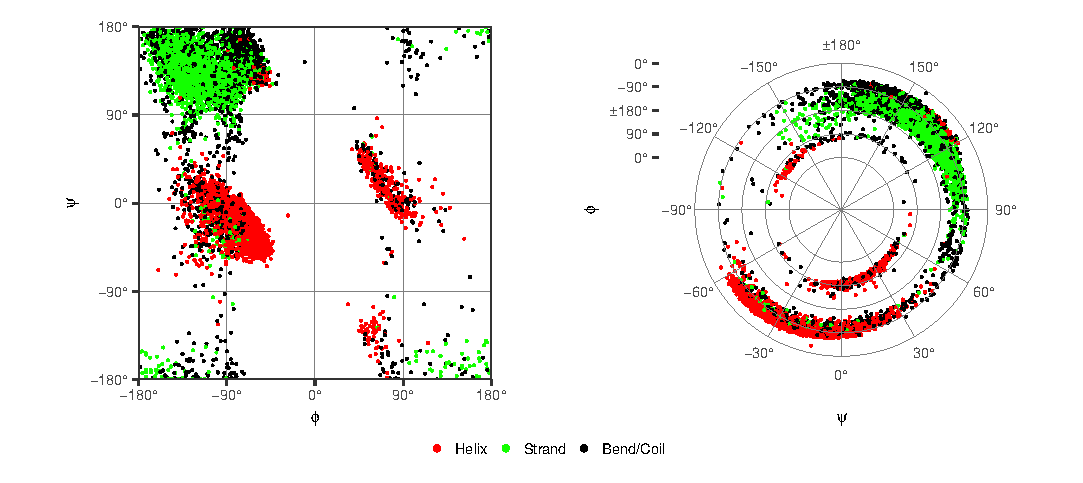
\includegraphics{Fig1}
\caption{{\bf Bold the figure title.}
Figure caption text here, please use this space for the figure panel descriptions instead of using subfigure commands. A: Lorem ipsum dolor sit amet. B: Consectetur adipiscing elit.}
\label{fig1}
\end{figure*}

% Results and Discussion can be combined.
\section*{Results}
Nulla mi mi, venenatis sed ipsum varius, Table~\ref{table1} volutpat euismod diam. Proin rutrum vel massa non gravida. Quisque tempor sem et dignissim rutrum. Lorem ipsum dolor sit amet, consectetur adipiscing elit. Morbi at justo vitae nulla elementum commodo eu id massa. In vitae diam ac augue semper tincidunt eu ut eros. Fusce fringilla erat porttitor lectus cursus, vel sagittis arcu lobortis. Aliquam in enim semper, aliquam massa id, cursus neque. Praesent faucibus semper libero.

% Place tables after the first paragraph in which they are cited.
\begin{table}[!ht]
\begin{adjustwidth}{-2.25in}{0in} % Comment out/remove adjustwidth environment if table fits in text column.
\centering
\caption{
{\bf Table caption Nulla mi mi, venenatis sed ipsum varius, volutpat euismod diam.}}
\begin{tabular}{|l+l|l|l|l|l|l|l|}
\hline
\multicolumn{4}{|l|}{\bf Heading1} & \multicolumn{4}{|l|}{\bf Heading2}\\ \thickhline
$cell1 row1$ & cell2 row 1 & cell3 row 1 & cell4 row 1 & cell5 row 1 & cell6 row 1 & cell7 row 1 & cell8 row 1\\ \hline
$cell1 row2$ & cell2 row 2 & cell3 row 2 & cell4 row 2 & cell5 row 2 & cell6 row 2 & cell7 row 2 & cell8 row 2\\ \hline
$cell1 row3$ & cell2 row 3 & cell3 row 3 & cell4 row 3 & cell5 row 3 & cell6 row 3 & cell7 row 3 & cell8 row 3\\ \hline
\end{tabular}
\begin{flushleft} Table notes Phasellus venenatis, tortor nec vestibulum mattis, massa tortor interdum felis, nec pellentesque metus tortor nec nisl. Ut ornare mauris tellus, vel dapibus arcu suscipit sed.
\end{flushleft}
\label{table1}
\end{adjustwidth}
\end{table}


%PLOS does not support heading levels beyond the 3rd (no 4th level headings).
\subsection*{\lorem\ and \ipsum\ nunc blandit a tortor}
\subsubsection*{3rd level heading} 
Maecenas convallis mauris sit amet sem ultrices gravida. Etiam eget sapien nibh. Sed ac ipsum eget enim egestas ullamcorper nec euismod ligula. Curabitur fringilla pulvinar lectus consectetur pellentesque. Quisque augue sem, tincidunt sit amet feugiat eget, ullamcorper sed velit. Sed non aliquet felis. Lorem ipsum dolor sit amet, consectetur adipiscing elit. Mauris commodo justo ac dui pretium imperdiet. Sed suscipit iaculis mi at feugiat. 

% Place figure captions after the first paragraph in which they are cited.
\begin{figure*}[!h]
\begin{adjustwidth}{-2.25in}{0in} % Comment out/remove adjustwidth environment if table fits in text column.
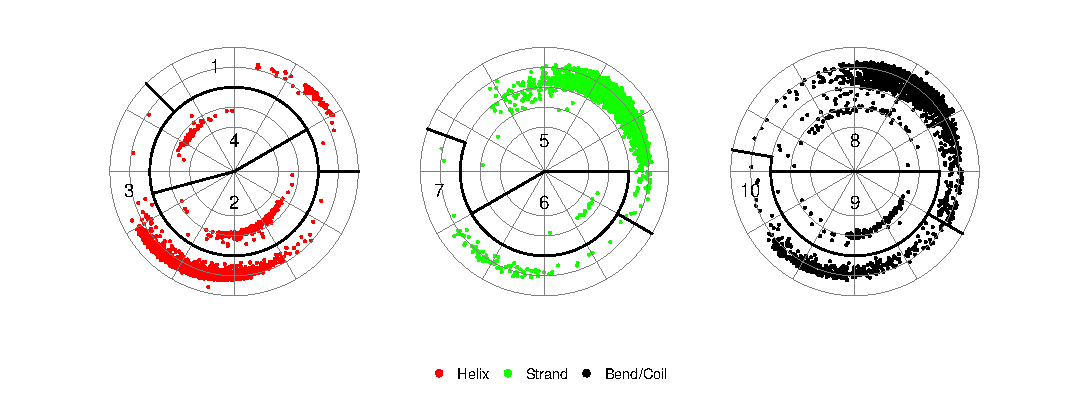
\includegraphics{Fig2}
\caption{{\bf Bold the figure title.}
Figure caption text here, please use this space for the figure panel descriptions instead of using subfigure commands. A: Lorem ipsum dolor sit amet. B: Consectetur adipiscing elit.}
\label{fig2}
\end{adjustwidth}
\end{figure*}

\begin{enumerate}
	\item{react}
	\item{diffuse free particles}
	\item{increment time by dt and go to 1}
\end{enumerate}


\subsection*{Sed ac quam id nisi malesuada congue}

Nulla mi mi, venenatis sed ipsum varius, volutpat euismod diam. Proin rutrum vel massa non gravida. Quisque tempor sem et dignissim rutrum. Lorem ipsum dolor sit amet, consectetur adipiscing elit. Morbi at justo vitae nulla elementum commodo eu id massa. In vitae diam ac augue semper tincidunt eu ut eros. Fusce fringilla erat porttitor lectus cursus, vel sagittis arcu lobortis. Aliquam in enim semper, aliquam massa id, cursus neque. Praesent faucibus semper libero.

\begin{itemize}
	\item First bulleted item.
	\item Second bulleted item.
	\item Third bulleted item.
\end{itemize}

\section*{Discussion}

Top-aligned is not ideal for containment searches. 


\section*{Conclusion}


\section*{Supporting information}

% Include only the SI item label in the paragraph heading. Use the \nameref{label} command to cite SI items in the text.
\paragraph*{S1 Fig.}
\label{S1_Fig}
{\bf Bold the title sentence.} Add descriptive text after the title of the item (optional).

\paragraph*{S2 Fig.}
\label{S2_Fig}
{\bf Lorem ipsum.} Maecenas convallis mauris sit amet sem ultrices gravida. Etiam eget sapien nibh. Sed ac ipsum eget enim egestas ullamcorper nec euismod ligula. Curabitur fringilla pulvinar lectus consectetur pellentesque.

\paragraph*{S1 File.}
\label{S1_File}
{\bf Lorem ipsum.}  Maecenas convallis mauris sit amet sem ultrices gravida. Etiam eget sapien nibh. Sed ac ipsum eget enim egestas ullamcorper nec euismod ligula. Curabitur fringilla pulvinar lectus consectetur pellentesque.

\paragraph*{S1 Video.}
\label{S1_Video}
{\bf Lorem ipsum.}  Maecenas convallis mauris sit amet sem ultrices gravida. Etiam eget sapien nibh. Sed ac ipsum eget enim egestas ullamcorper nec euismod ligula. Curabitur fringilla pulvinar lectus consectetur pellentesque.

\paragraph*{S1 Appendix.}
\label{S1_Appendix}
{\bf Lorem ipsum.} Maecenas convallis mauris sit amet sem ultrices gravida. Etiam eget sapien nibh. Sed ac ipsum eget enim egestas ullamcorper nec euismod ligula. Curabitur fringilla pulvinar lectus consectetur pellentesque.

\paragraph*{S1 Table.}
\label{S1_Table}
{\bf Lorem ipsum.} Maecenas convallis mauris sit amet sem ultrices gravida. Etiam eget sapien nibh. Sed ac ipsum eget enim egestas ullamcorper nec euismod ligula. Curabitur fringilla pulvinar lectus consectetur pellentesque.

\section*{Acknowledgments}
Cras egestas velit mauris, eu mollis turpis pellentesque sit amet. Interdum et malesuada fames ac ante ipsum primis in faucibus. Nam id pretium nisi. Sed ac quam id nisi malesuada congue. Sed interdum aliquet augue, at pellentesque quam rhoncus vitae.

\nolinenumbers

% Either type in your references using
% \begin{thebibliography}{}
% \bibitem{}
% Text
% \end{thebibliography}
%
% or
%
% Compile your BiBTeX database using our plos2015.bst
% style file and paste the contents of your .bbl file
% here. See http://journals.plos.org/plosone/s/latex for 
% step-by-step instructions.
% 
%\begin{thebibliography}{10}


%\end{thebibliography}

\bibliography{rupee}

\end{document}

